%% Copyright 1998 Pepe Kubon
%%
%% `two.tex' --- 2nd chapter for thes-full.tex, thes-short-tex from
%%               the `csthesis' bundle
%%
%% You are allowed to distribute this file together with all files
%% mentioned in READ.ME.
%%
%% You are not allowed to modify its contents.
%%

%%%%%%%%%%%%%%%%%%%%%%%%%%%%%%%%%%%%%%%%%%%%%%%%%
%
%     Chapter 6  
%
%%%%%%%%%%%%%%%%%%%%%%%%%%%%%%%%%%%%%%%%%%%%%%%%

\chapter{Experiments}
\label{ch:exp}

To validate the efficiency of our two methods named GP and MHI, we first report the experimental results with respect to Jaccard similarity on synthetic data sets in Section~\ref{sec:syn-data}. The results on two real data sets on market basket data and click stream data are presented in Section~\ref{sec:real-data}. We also show the performance of the pruning algorithms on Cosine similarity and edit distance in Section~\ref{sec:other-measure} using the click stream data set. All methods are implemented in Python and all experiments are conducted on a PC computer with Intel Core 2 Duo E8400 3.00GHz CPU and 8GB main memory running 64-bit Microsoft Windows 7.


%%%%%% Synthetic Data Set %%%%%%
\section{Results on Synthetic Data Sets}
\label{sec:syn-data}
The following results are generated using the IBM Quest data generator\footnote{\url{http://www.cs.loyola.edu/~cgiannel/assoc_gen.html}}. We conduct experiments to test the efficiency and accuracy of our methods regarding the following parameters. 
% We use the following notations for ease of presentation: 

\begin{itemize}
\item $k$ - top-$k$; 
\item $n$ - number of items per query/ average number of items per object.
\item $|\Sigma|$ - lexicon size;
\item $m$ - number of objects;
\item $l$ - number of different hash functions/ random permutations.
\end{itemize}

%%% test on IBM Quest data %%%

\begin{figure*}[htb]
\centering
\subfigure{% a
\label{legend}

\includegraphics[width=1\textwidth]{fig/legend_efficiency.eps}}
\quad
\setcounter{subfigure}{0}
\subfigure[Large $|\Sigma|$]{% a
\label{questLLVka}
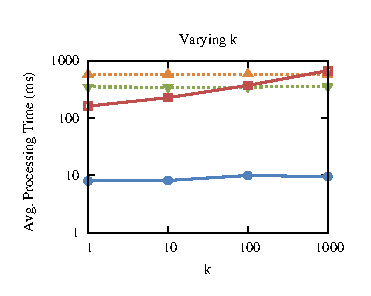
\includegraphics[width=0.45\textwidth]{fig/vary_k_large.eps}}
\quad
\subfigure[Small $|\Sigma|$]{% b
\label{questSLVka}
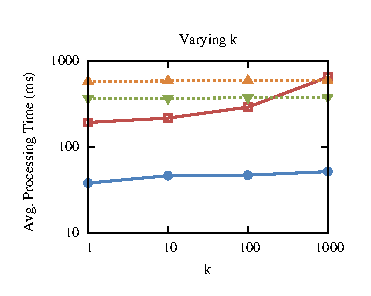
\includegraphics[width=0.45 \textwidth]{fig/vary_k_small.eps}}
\quad
\subfigure[]{% c
\label{questVsigmaa}
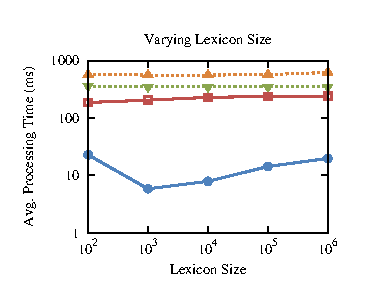
\includegraphics[width=0.45 \textwidth]{fig/vary_lexicon.eps}}
\quad
\subfigure[]{% g
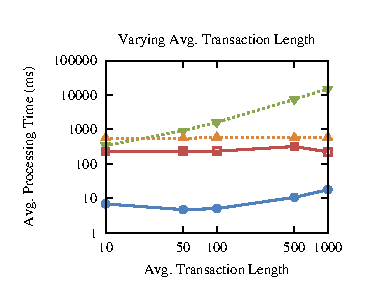
\includegraphics[width=0.45 \textwidth]{fig/vary_txn_len.eps} 
\label{questVna}}
\quad
\subfigure[]{% h
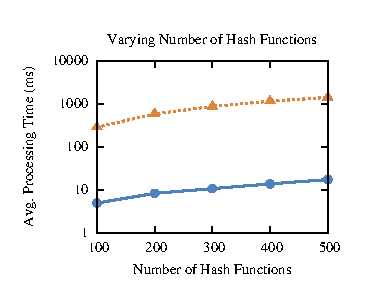
\includegraphics[width=0.45 \textwidth]{fig/vary_l.eps} 
\label{questVla}}
\quad
\subfigure[]{% i
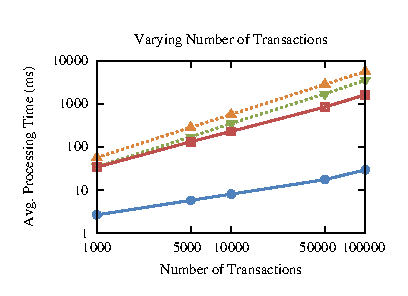
\includegraphics[width=0.45 \textwidth]{fig/vary_m.eps} 
\label{questVma}}

\caption{Average Processing Time on IBM Quest Data Set Using Jaccard Similarity}
\label{ibmTestsAvgEff}
\end{figure*}

\begin{figure*}[htb]
\centering
\subfigure[Large $|\Sigma|$]{% d
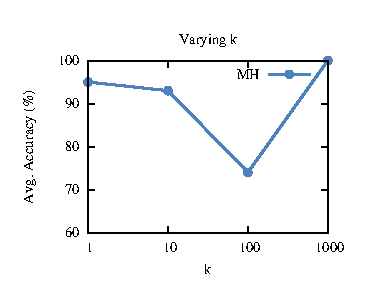
\includegraphics[width=0.45 \textwidth]{fig/acc_vary_k_large.eps} 
\label{questLLVkb}}
\quad
\subfigure[Small $|\Sigma|$]{% e
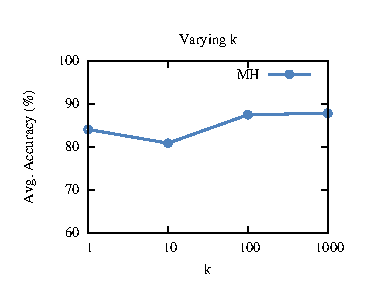
\includegraphics[width=0.45 \textwidth]{fig/acc_vary_k_small.eps} 
\label{questSLVkb}}
\quad
\subfigure[]{% f
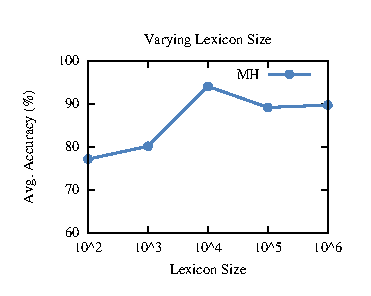
\includegraphics[width=0.45 \textwidth]{fig/acc_vary_lexicon.eps} 
\label{questVsigmab}}
\quad
\subfigure[]{% j
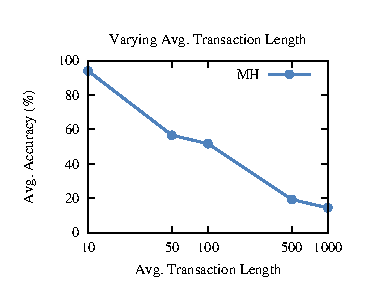
\includegraphics[width=0.45 \textwidth]{fig/acc_vary_tlen.eps} 
\label{questVnb}}
\quad
\subfigure[]{% k
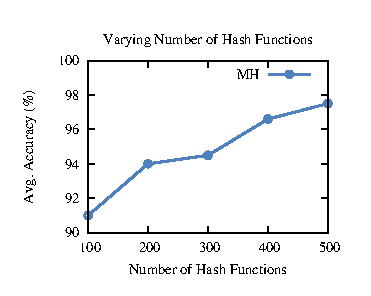
\includegraphics[width=0.45 \textwidth]{fig/acc_vary_l.eps} 
\label{questVlb}}
\quad
\subfigure[]{% l
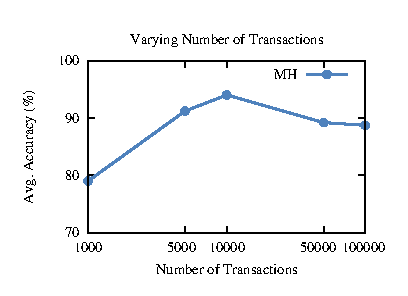
\includegraphics[width=0.45 \textwidth]{fig/acc_vary_m.eps} 
\label{questVmb}}
\caption{Average Accuracy of Hashing-based Method on IBM Quest Data Set Using Jaccard Similarity}
\label{ibmTestsAvgAcc}
\end{figure*}


\begin{figure*}[htb]
\centering
\subfigure[Large $|\Sigma|$]{% g
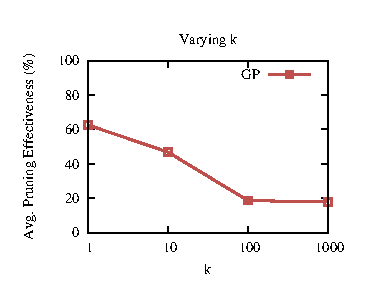
\includegraphics[width=0.45 \textwidth]{fig/preff_vary_k_large.eps} 
\label{questVkPreffL}}
\quad
\subfigure[Small $|\Sigma|$]{% h
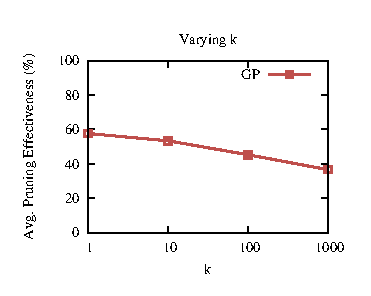
\includegraphics[width=0.45 \textwidth]{fig/preff_vary_k_small.eps} 
\label{questVkPreffS}}
\quad
\subfigure[]{% k
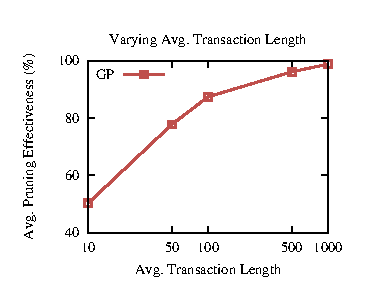
\includegraphics[width=0.45 \textwidth]{fig/preff_vary_tlen.eps} 
\label{questVnPreff}}
\quad
\subfigure[]{% j
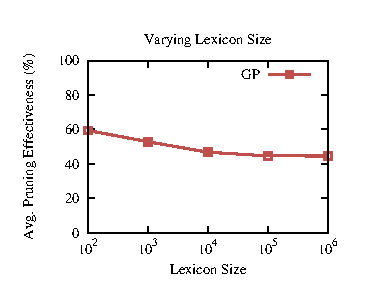
\includegraphics[width=0.45 \textwidth]{fig/preff_vary_lexicon.eps} 
\label{questVsigmaPreff}}
\quad
\raggedright
\subfigure[]{% i
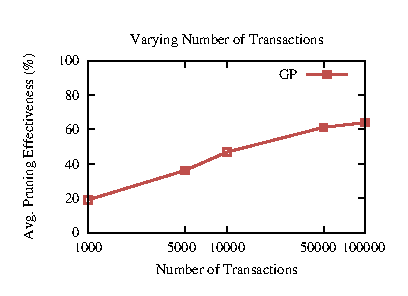
\includegraphics[width=0.45 \textwidth]{fig/preff_vary_m.eps} 
\label{questVmPreff}}
\caption{Pruning Effectiveness of GP on IBM Quest Data Set Using Jaccard Similarity}
\label{ibmTestsP3}
\end{figure*}


%Let us denote Algorithm~\ref{minHashBasic} as ``MHB'', which can be regarded as the baseline for hash-based algorithms. Algorithm~\ref{minHashInd} is named as ``MHI". Our first pruning-based algorithm is denoted as ``GP". 
To generate synthetic datasets using the IBM Quest data generator, we set parameters for $n$, $|\Sigma|$, and $m$. The synthetic query stream is generated by concatenating random objects whose lengths are between $0.8\bar{n}$ to $1.2\bar{n}$, where $\bar{n}$ is the average object length of the data set. In reality, the distribution of the elements in the stream would not change much in a very short time period. For example, on a Q\&A forum, some hot topics and its related ones may be discussed heavily for an hour before moving to the next groups of hot topics. In terms of average querying time, comparing to the real scenario, the performance of our algorithms using the generated query stream may be slower. It is because in our way of generating the stream, the transit from one topic to another is relatively faster than the typical real case.

We use the variable controlling method to conduct our experiments. The values of controlled variables along with the corresponding figures for each test are shown in Table~\ref{defaultVal}. In each variable controlled test, we compare the performance of GP and MHI, on the average querying time with two baseline methods, namely, BFM and MHB. BFM is a brute-force method that computes the exact similarity scores for every object with respect to a query. MHB is a baseline method based on MinHash technique but without indexing structures. To better illustrate how our upper bounds derived in Chapter~\ref{ch:pruning} can be used to prune unpromising objects, we define the pruning effectiveness of an update in Definition~\ref{preff-def}. In our experiments, we report the average pruning effectiveness of hundreds of updates. 

\begin{definition}[Pruning Effectiveness of Pruning-based Method]\label{preff-def}
Suppose we have $m$ objects in total and we compute the exact similarity scores for $m^*$ objects during an update. The pruning effectiveness of this update is $1 - \frac{m^*}{m}$. 
\end{definition}

The \emph{accuracy} in our context is defined in Definition~\ref{acc-methods}. The pruning algorithm GP always reports the exact query results, which has $100\%$ accuracy. However, since the MinHash-based methods compute similarity scores approximately, MHB and MHI give estimated answers to the top-$k$ query. We report the average accuracy of MinHash methods in Figure~\ref{ibmTestsAvgAcc}. 

\begin{definition}[Accuracy of a Method]\label{acc-methods}
Suppose the exact top-$k$ list regarding query $q_t$ is $top_k^{e}$ and the $k$-th best object is denoted as $o_{r_k}^e$. Given a method $A$ that returns a top-$k$ list, $top_k^A$, regarding query $q_t$, the accuracy of method $A$ is the proportion of objects in $top_k^A$ whose exact similarity scores regarding $q_t$ is no smaller than the $k$-th best similarity score in $top_k^{e}$. More formally, $acc_A$, the accuracy of method $A$ for $q_t$ is defined as $$acc_A = \frac{|\{o|o \in top_k^A \land sim(o, q_t)\geq sim(o_{r_k}^e, q_t)\}|}{k}\text{.}$$
\end{definition}

\begin{table}[t]
\caption{Values of Controlled Variables for Tests on Jaccard Similarity}  
\label{defaultVal} 
%\setlength{\tabcolsep}{0.5\tabcolsep}
\begin{center}%\resizebox{70mm}{!}
{
    \begin{tabular}{ |c|c|c|c|c|c|c|}
    \hline
    Test  & $k$ & $n$ & $|\Sigma|$ & $l$& $m$ &Figures\\ \hline
    Synthetic Data (Vary $k$) & n/a  &  $10$ & $10,000$  & $200$ & $10,000$  & Fig.~\ref{questLLVka}, \ref{questLLVkb}\\ \hline
    Synthetic Data (Vary $k$) & n/a &  $10$ &  $20$ & $200$ & $10,000$ & Fig.~\ref{questSLVka}, \ref{questSLVkb}\\ \hline
    Synthetic Data (Vary $|\Sigma|$) & $10$ &  $10$ &  n/a & $200$ & $10,000$  & Fig.~\ref{questVsigmaa}, \ref{questVsigmab}\\ \hline
    Synthetic Data (Vary $n$) & $10$ &  n/a &  $10,000$ & $200$ & $10,000$  & Fig.~\ref{questVna}, \ref{questVnb}\\ \hline
    Synthetic Data (Vary $l$) & $10$ &  $10$ &  $10,000$ & n/a & $10,000$  & Fig.~\ref{questVla}, \ref{questVlb}\\ \hline
    Synthetic Data (Vary $m$) & $10$ &  $10$ & $10,000$ & $200$ &  n/a   & Fig.~\ref{questVma}, \ref{questVmb}\\ \hline
    Market Basket (Vary $l$) & $10$ &  $10$ & $16,470$ & n/a &  $88,162$   & Fig.~\ref{mbdsVlTime}, \ref{mbdsVlAcc}\\ \hline
    Market Basket (Vary $k$) & n/a &  $10$ & $16,470$ & $200$ &  $88,162$   & Fig.~\ref{mbdsVkTime}, \ref{mbdsVkAcc}\\ \hline
    Click Stream (Vary $l$) & $10$ &  $5$ & $17$ & n/a &  $31,790$   & Fig.~\ref{msnbcVlTime}, \ref{msnbcVlAcc}\\ \hline
    Click Stream (Vary $k$) & n/a &  $5$ & $17$ & $50$ &  $31,790$   & Fig.~\ref{msnbcVkTime}, \ref{msnbcVkAcc}\\ \hline
    \end{tabular}}
\end{center}
%\setlength{\tabcolsep}{2\tabcolsep}
\end{table}

\subsection{Efficiency}    
The average querying time of the four methods when $k$ varies is shown in Figures~\ref{questLLVka} and \ref{questSLVka} for two synthetic data sets with large lexicon ($10^4$) and small lexicon ($20$), respectively. We can observe that in both cases, the two baseline methods almost have no change in average processing time and MHI that uses $200$ hash functions outperforms the other three methods greatly. The pruning effectiveness of GP is shown in Figure~\ref{questVkPreffL} and Figure~\ref{questVkPreffS} when the lexicon size is set to $10^4$ and $20$, respectively. GP's pruning power drops gradually because the similarity score of the $k$-th best object in the top-$k$ result tends to decrease when $k$ increases. Given other parameters fixed, the similarity score of the $k$-th best object in the result with respect to queries would be smaller. Thus, the pruning effectiveness generally is weaker in the case of larger lexicon size. 

Figure~\ref{questVsigmaa} provides a better illustration of the trends of different methods when the lexicon size changes. When the lexicon size increases by orders of magnitude, we can see that the pruning effectiveness drops from $59.4\%$ to $44.5\%$ gradually. Thus, the average processing time of GP increases. The average running time of MHB and BFM does not have obvious change with respect to lexicon size. However, the average running time of MHI first decreases and then increases. When the lexicon size is small, the length of each inverted list is relatively large. Thus, a change in MinHash value of the query may result in many updates in the estimated similarity scores. When lexicon size becomes very large, though the size of each inverted list is small, the number of unmatched MinHash values between the MinHash lists of the previous query and the new query increases, which results in more queries on the inverted indices. 

We also examine how the average query answering time changes with respect to average object length. The results on efficiency and pruning effectiveness are shown in Figures~\ref{questVna}, and~\ref{questVnPreff}. The average processing time of BFM increases linearly while the performance of MHB does not have obvious change with respect to average object length. It is because we have transformed the transctions of varied length into MinHash signatures of the same length. However, the average processing time of MHI first decreases slightly and then increases. When the average object length becomes larger, the size of each inverted list would be larger, which results in longer processing time. When the average object length increases, the pruning effectiveness of GP increases dramatically, from $46.8\%$ to $97.2\%$. However, its average running time still increases slightly, since there is an increase in computing exact similarity scores for larger sets in the verification phase.   
% reaches the minimum when the average transaction length is $10$.
% Done - Add: analyze MHI 

The results with respect to the number of hash functions is shown in Figure~\ref{questVla}.  The average processing time of MHB and MHI both increases linearly with the number of hash functions, which is in accordance with the analysis of our algorithms.  The scalability of three methods is shown in Figure~\ref{questVma}.  All the methods increases linearly as the number of object increases.  The pruning power of GP increases from $19.1\%$ to $64.0\%$ when the number of objects increases from $10^3$ to $10^5$, which is shown in Figure~\ref{questVmPreff}.   
% Done - Add: describe scalability 

\subsection{Accuracy}
We also test the accuracy of the MinHash-based algorithms. By our definition, the accuracy of the two MinHash-based algorithms are the same according to the same set of hash functions. We denote the MinHash methods by MH in the figures that report accuracy. The accuracy can be affected by two factors, the number of hash functions used and the intrinsic characteristics of our data set such as the distribution of similarity scores among objects. 
% For example, if there are many objects with close similarity scores to those of objects in the exact top-$k$ list, then the accuracy tends to be lower. 

In general, we can achieve an accuracy ranging from $70\%$ to $98\%$ when $200$ hash functions are used. Figures~\ref{questLLVkb} and~\ref{questSLVkb} show the change in accuracy when $k$ increases for data sets with large lexicon and small lexicon, respectively. In the case where lexicon size is $10^4$, the accuracy first decreases and then increases. The smallest average accuracy rate is achieved when $k = 10^2$. When $k$ is very large, say $10^3$, the $k$-th best similarity score would become $0$, which is the reason why the accuracy increases to $100\%$ when $k$ is $10^3$. This issue does not occur in the case of small lexicon. When lexicon size is $20$, we can achieve accuracy in the range of $80\%$ to $88\%$. The average accuracy first decreases and then increases, and the smallest average accuracy rate is achieved when $k = 10$.   

%%% test on retail.txt %%%
\begin{figure*}[htb]
\centering
\subfigure{% a
\label{legend}

\includegraphics[width=1\textwidth]{fig/legend_efficiency.eps}}
\quad
\setcounter{subfigure}{0}
\subfigure[]{% i
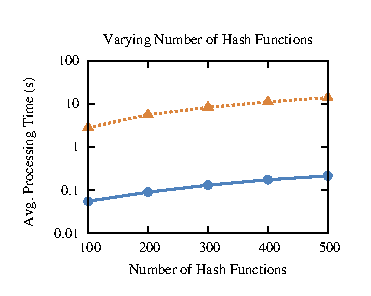
\includegraphics[width=0.45 \textwidth]{fig/rmarket_vary_l.eps} 
\label{mbdsVlTime}}
\quad
\subfigure[]{% j
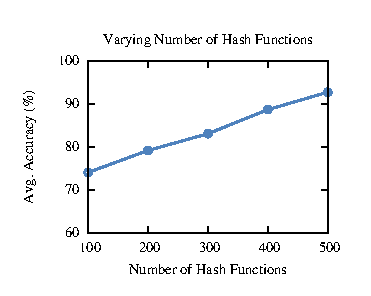
\includegraphics[width=0.45 \textwidth]{fig/rmarket_acc_vary_l.eps} 
\label{mbdsVlAcc}}
\quad
\subfigure[]{% g
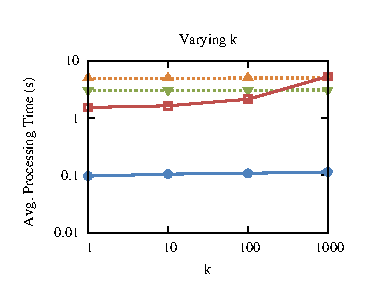
\includegraphics[width=0.45 \textwidth]{fig/rmarket_vary_k.eps} 
\label{mbdsVkTime}}
\quad
\subfigure[]{% h
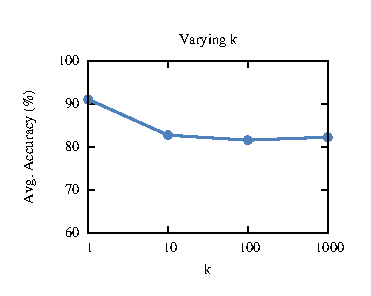
\includegraphics[width=0.45 \textwidth]{fig/rmarket_acc_vary_k.eps} 
\label{mbdsVkAcc}}
\quad
\raggedright
\subfigure[]{% i
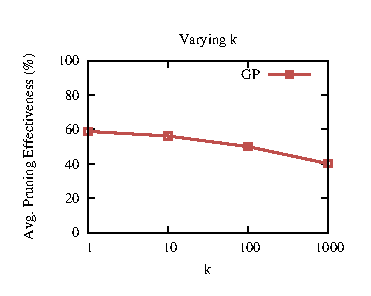
\includegraphics[width=0.45 \textwidth]{fig/rmarket_preff_vary_k.eps} 
\label{mbdsVkPreff}}
\caption{Results on Market Basket Dataset Using Jaccard Similarity}
\label{mbData}
\end{figure*}


The average accuracy increases quickly and then decreases slightly when the lexicon size increases, which is shown in Figure~\ref{questVsigmab}.  The highest accuracy is achieved when lexicon size is $10^4$.  In Figure~\ref{questVnb}, when the average object length increases from $10$ to $10^3$, the accuracy drops drastically from $94\%$ to $14.4\%$.  The reason is apparent.  More hash functions are needed to achieve the same level of accuracy when the set size gets larger. 
% Done - Correct: first sentence not consistent now

We also test the trend of accuracy when the number of hash functions and the number of objects increase.  The results are shown in Figures~\ref{questVlb} and \ref{questVmb}, respectively.  When more hash functions are used, the estimated Jaccard similarity is closer to the exact score, thus lead to higher accuracy.  As shown in Figure~\ref{questVlb}, we can see that the result follows this trend and we can achieve average accuracy rate ranging from $91\%$ to $97.5\%$.  Figure~\ref{questVmb} suggests that the average accuracy first increases and then decreases when the number of objects increases. The highest accuracy is achieved when $m = 10^4$.  

%%%%%% Real Data Set %%%%%%
\section{Results on Real Data Sets}
\label{sec:real-data}

\begin {table}[t]
\caption {Real Data Sets Statistics}  
%\setlength{\tabcolsep}{0.5\tabcolsep}
\label{datasetStat} 
\begin{center}%\resizebox{70mm}{!}
{
    \begin{tabular}{ |c|c|c|c|}
    \hline
    Data Set  & Cardinality & Avg. Length & Lexicon Size \\ \hline
    Market Basket & 88,162 & 10.306 & 16,470 \\ \hline
    MSNBC & 31,790 & 5.3338 & 17 \\ \hline
    \end{tabular}}
\end{center}
%\setlength{\tabcolsep}{2\tabcolsep}
\end {table}

We conduct experimental studies on two real data sets: a retail market basket data set\footnote{\url{http://fimi.ua.ac.be/data/}} from an anonymous Belgian retail store and MSNBC, a data set of click-stream data. We use a subset of the MSNBC data set that removes the shortest sequences, with the link provided \footnote{\url{http://www.philippe-fournier-viger.com/spmf/}}. We then transform each sequence into set. There is a significant difference in lexicon size of the two real data sets. The market basket data set has $16,470$ distinct items while the MSNBC data set contains only $17$ distinct items. Table~\ref{datasetStat} shows the detailed statistics of the data sets. To generate the querying stream, we randomly concatenate objects in the data set whose size is between $0.8\bar{n}$ to $1.2\bar{n}$, where $\bar{n}$ is the average object length of the data set. For each data set, we compare the average processing time and the average accuracy when $k$ or $l$ varies, respectively. The results are shown in Figure~\ref{mbData} and \ref{csData}. 

The trends of the curves for the market basket data set is highly consistent with the results on the synthetic data sets. In Figure~\ref{mbdsVlTime} and \ref{mbdsVlAcc}, we show the trends of processing time and accuracy of the MinHash based methods when different number of hash functions is used.  The average processing time of MHB and MHI both increases linearly with the number of hash functions.  The performance of MHI is around $50$ to $65$ times faster than MHB.  The average accuracy increases steadily from $74\%$ to $93\%$ when the number of hash functions increases from $100$ to $500$.  To compare the average processing time of different methods, we choose the default number of hash functions as $200$.  The processing time of BFM, MHB, and MHI does not have obvious change and MHI always has the best performance.  The pruning power of GP decreases from $60\%$ to $40\%$ gradually when $k$ increases.  Therefore, the processing time of GP increases when $k$ increases.  The MinHash based algorithms can achieve accuracy over $80\%$ when $k$ is varied from $1$ to $1000$, which is shown in Figure~\ref{mbdsVkAcc}. 

The results for the click stream data set is shown in Figure~\ref{csData}.  Since the average length of the objects in this data set is only $5.33$, the MinHash based algorithms do not need many hash functions in order to achieve very high accuracy.  As shown in Figure~\ref{msnbcVlAcc}, the average accuracy is above $90\%$ when over $30$ hash functions are used.  To test the preformance when $k$ varies, we use $30$ hash functions. MHI is still the best method with respect to average query answering time, which can outperform the BFM by more than an order of magnitude. Comparing to the results on market basket data set, the average accuracy of MinHash-based methods is generally higher while the pruning effectiveness of GP is lower for the click stream data set.  
% Done - Add: discuss the special case       



%%% test on msnbcSubSet.txt %%%
\begin{figure*}[htb]
\centering
\subfigure{% a
\label{legend}

\includegraphics[width=1\textwidth]{fig/legend_efficiency.eps}}
\quad
\setcounter{subfigure}{0}
\subfigure[]{% i
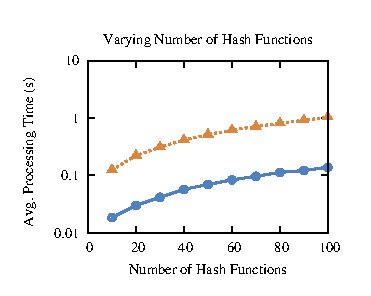
\includegraphics[width=0.45 \textwidth]{fig/rclicks_vary_l.eps} 
\label{msnbcVlTime}}
\quad
\subfigure[]{% j
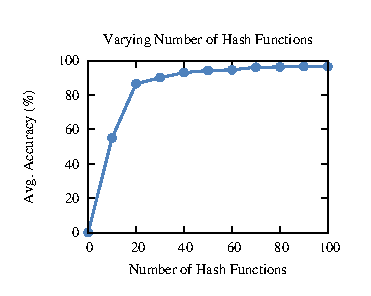
\includegraphics[width=0.45 \textwidth]{fig/rclicks_acc_vary_l.eps} 
\label{msnbcVlAcc}}
\quad
\subfigure[]{% g
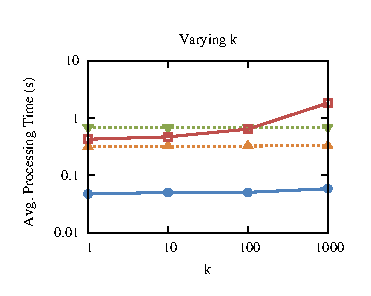
\includegraphics[width=0.45 \textwidth]{fig/rclicks_vary_k.eps}   
\label{msnbcVkTime}} 
\quad
\subfigure[]{% h 
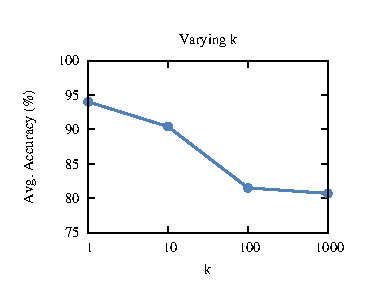
\includegraphics[width=0.45 \textwidth]{fig/rclicks_acc_vary_k.eps} 
\label{msnbcVkAcc}}
\quad
\raggedright
\subfigure[]{% i
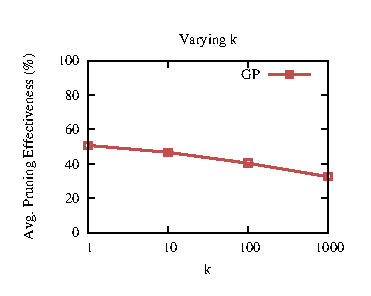
\includegraphics[width=0.45 \textwidth]{fig/rclicks_preff_vary_k.eps} 
\label{msnbcVkPreff}}

\caption{Results on Click Stream Dataset Using Jaccard Similarity}
\label{csData}
\end{figure*}

\section{Results on Other Similarity Measures}
\label{sec:other-measure}
In this section, we experiment on the performance of the bounds, derived in Section~\ref{sec:gen-sim}, for cosine similarity and edit similarity, using the click stream data set.  Since cosine similarity can be approximated using a random projection method~\cite{C02}, we can use the hashing-based framework for Jaccard similarity only with the signature generation phase changed. The random projection method chooses random hyperplanes defined by normal unit vectors and uses the signs of the dot products between the input vector and random hyperplanes as the signature for this vector. Given the signatures of two vectors generated by the same set of random hyperplanes, the percentage of matching bits in their signatures is proportional to the cosine distance between two vectors. Corresponding to MHB and MHI for Jaccard similarity, the hashing-based methods for cosine similarity are denoted as RPB and RPI. By default, we use $200$ random hyperplanes in our experiment.

The results for cosine similarity is shown in Figure~\ref{msnbcCos}.  The pruning effectiveness decreases from $86.0\%$ to $78.6\%$ when $k$ varies from $1$ to $1000$.  It is apparant since our similarity bound depends on the $k^{th}$ best score.  When $k$ increases, the $k^{th}$ best score decreases, thus less objects can be pruned. The average processing time increases when $k$ increases, which is in accordance with the trend of the pruning effectiveness. The pruning-based method has better performance, in terms of both querying time and accuracy, than the hashing-based method. We should notice that signatures constructed by random projection method only consist of $0$ and $1$. Since we use inverted indices in the same way as for Jaccard similarity, the number of objects in each inverted list would be very large. It can be the reason why the performance of the hashing-based algorithm becomes worse for cosine similarity.  

Figure~\ref{msnbcEd} shows the results for edit similarity on click stream data set. The trend is similar to that of cosine similarity and Jaccard similarity.  The algorithm can prune $64.8\%$ to $46.8\%$ objects when $k$ increases from $1$ to $100$.  Among the three distance measures, the bound for cosine similarity has the best pruning effectiveness; The bound for edit similarity comes second and the bound for Jaccard similarity is slightly worse than that of edit similarity.   
     
% Done - Add

\section{Summary of Results}
We conduct experiments to test the effectiveness and efficiency of our pruning-based method and hashing-based method. There are $5$ parameters that can affect the performance of our methods. We test our methods by varying one parameter in each test and compare the performance of our methods. 

Generally speaking, in terms of accuracy, the pruning-based method is an exact method while the hashing-based method can reach very good accuracy rate when a few hundreds of hash functions are used. For Jaccard similarity, the hashing-based method with good accuracy results can always achieve faster average querying time than the pruning-based method. However, for cosine similarity, the pruning method can achieve better performance than the hashing-based method. One reason is that the pruning effectiveness of cosine similarity is the highest among the three similarity measures in our experiments. The other reason is that the inverted indices can not reduce much work in updating the similarity scores since each inverted list can be very long with length equals to half of the number of transactions on average. 




% However, the accuracy rate is sensitive to the average number of items per object. For example, to achieve the same level of accuracy, we need $50$ hash functions when $n = 5$ while $100$ hash functions are required when $n = 10$. The performance of the pruning-based method is highly related to the similarity score between the evolving query and the $k^{th}$ best object in the top-$k$ result. If this score is very large while the similarity between the query and each object that are not currently in the top-$k$ result is very small, then we only need to compute a tiny portion of exact similarity scores in each update. 



% Let us consider an extreme case. If only a few number (close to $k$) of objects are very similar to the query and the other objects are very different, then we only need to compute a tiny portion of exact similarity scores in each update.  

%%% test on msnbcSubSet.txt for cosine sim %%%
%\vspace{-5 mm}
\begin{figure*}[htb]
\centering
\subfigure{% a
\label{legend}

\includegraphics[width=1\textwidth]{fig/legend_efficiency_rp.eps}}
\vspace{-5 mm}
\quad
\setcounter{subfigure}{0}
\subfigure[]{% d
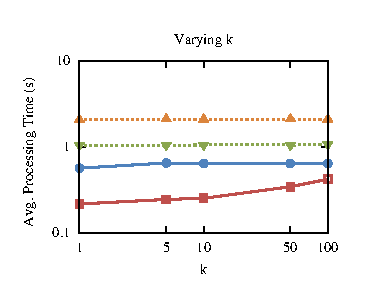
\includegraphics[width=0.445 \textwidth]{fig/rclicks_vary_k_cos.eps} 
%\label{msnbcVkCos}}
}
\quad
\subfigure[]{% e
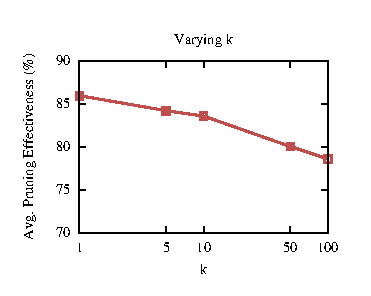
\includegraphics[width=0.445 \textwidth]{fig/rclicks_preff_vary_k_cos.eps} 
%\label{msnbcVkPreffCos}}
}
\quad 
\raggedright
\subfigure[]{% e
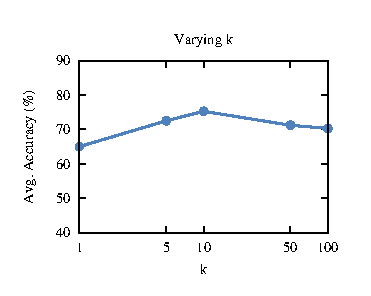
\includegraphics[width=0.445 \textwidth]{fig/rclicks_acc_vary_k_cos.eps} 
\label{msnbcVkAccCos}}
\vspace{-3mm}
\caption{Results on Click Stream Dataset Using Cosine Similarity}
\label{msnbcCos}
\end{figure*}
\vspace{-10 mm}
\begin{figure*}[htb]
\centering
\subfigure[]{% d
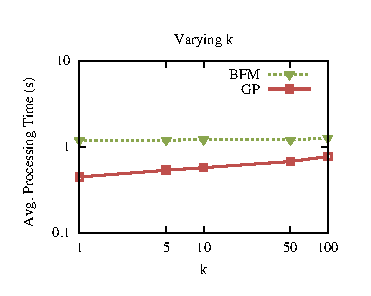
\includegraphics[width=0.445 \textwidth]{fig/rclicks_vary_k_ed.eps} 
\label{msnbcVkEd}}
\quad
\subfigure[]{% e
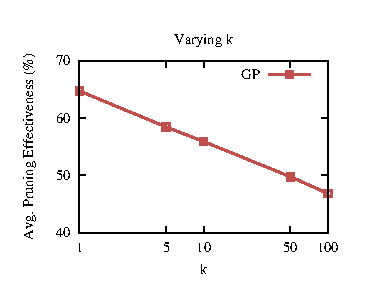
\includegraphics[width=0.445 \textwidth]{fig/rclicks_preff_vary_k_ed.eps} 
\label{msnbcVkPreffEd}}
\vspace{-3mm}
\caption{Results on Click Stream Dataset Using Edit Similarity}
\label{msnbcEd}
\end{figure*}

%\vspace{3 mm}


% Thus, the similarity score distribution in the data set and the number of similar objects we want to find. Although the   

% More specifically, there are $5$ parameters that can affect the performance of our methods, including the number of similar objects to select ($k$), lexicon size ($|\Sigma|$), average number of items per transaction ($n$), number of objects ($m$), and number of hash functions used ($l$). We test our methods by varying only one of the above parameters each time.   

    
